\section{Bezpieczeństwo}
% Porównanie bezpieczeństwa algorytmów RSA i ECC w zastosowaniu na aktualnymi technologiami

% Jak porównywać bezpieczeństwo algorytmów
\begin{frame}{Porównywanie bezpieczeństwa}
\textbf{Bity bezpieczeństwa \cite{BitSecurityOfCryptographicPrimitives}}
\begin{itemize}
    \pause
    \item Pojedyncza liczba
    \pause
    \item \( x = \log_2(N) \)
    \item \( x \) - liczba bitów bezpieczeństwa
    \item \( N \) - średnia ilość operacji wymaganych do złamania szyfru
\end{itemize}
\pause
\vspace{8mm}

\textit{Algorytm o sile 20 bitów bezpieczeństwa wymaga średnio $2^{20} = 1048576$ operacji do złamania.}

\end{frame}

\begin{frame}{Bezpieczeństwo RSA}
% Wielkość klucza to ilość bitów modułu n = p*q
Najszybszy klasyczny \footnote{tz. nie korzystający z matematyki kwantowej} algorytm refaktoryzacji liczb to Ogólne sito ciała liczbowego (GNFS) \footnote{ang. General Number Field Sieve}.
\begin{itemize}
    \item Złożoność \cite{GNFSImplementation} \begin{footnotesize}$$L(n) = \exp\left(\left(\frac{64}{9}\right)^{1/3} (\ln n)^{1/3} (\ln \ln n)^{2/3}\right)$$\end{footnotesize}
    \item Liczba bitów bezpieczeństwa $= \log_2(L(n))$
\end{itemize}
\pause
$$
\begin{array}{|c|c|}
\hline
\textbf{Wielkość \, klucza \, RSA \, (bity)} & \textbf{Bity \, Bezpieczeństwa} \\
\hline
1024 & \sim 80 \\
2048 & \sim 112 \\
3072 & \sim 128 \\
\hline
\end{array}
$$
\end{frame}

\begin{frame}{Bezpieczeństwo ECC}
% Wielkość klucza to rozmiar jednego wymiaru dyskretnej przestrzeni
Najszybszy klasyczny \footnote{tz. nie korzystający z matematyki kwantowej} algorytm do rozwiązania ECDLP to algorytm faktoryzacji rho Pollarda \cite{SolvingECDLP}.
\begin{itemize}
    \item Dla przestrzeni wielkości k wymaga $\sqrt{k}$ kroków
    \item Do x bitów bezpieczeństwa potrzebny jest klucz wielkości 2x
    \item Przykładowo 256-bitowa krzywa teoretycznie daje 128-bitów bezpieczeństwa
\end{itemize}
\pause
Rzeczywiste bezpieczeństwo $\approx 0.886*\sqrt{k}$
\pause
\begin{itemize}
    \item \textit{secp256k1} klucz 256 bit $\Rightarrow$ 127.8 bitów bezpieczeństwa \cite{Secp256k1Security}
    \item \textit{Curve448} klucz 448 bit $\Rightarrow$ 222.8 bitów bezpieczeństwa \cite{Secp256k1Security}
\end{itemize}
% Rzeczywiste bezpieczeństwo jest mniejsze, ponieważ ranga krzywej w dyskretnej przestrzeni jest zazwyczaj mniejsza niż wielkość pojedynczego wymiaru przestrzeni

\end{frame}

\begin{frame}{Porówanie długości klucza}
    \begin{figure}
        \centering
            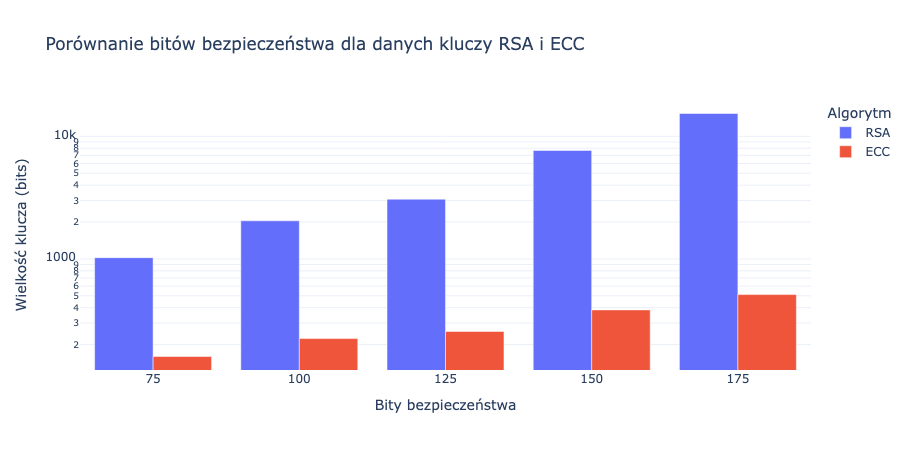
\includegraphics[width=\textwidth]{security/graphics/Porównanie bitów bezpieczeństwa dla danych kluczy RSA i ECC}
            \caption{Porównanie bitów bezpieczeństwa dla danych kluczy RSA i ECC}
    \end{figure}
\end{frame}

\begin{frame}{Problem wyboru krzywej ECC}
    % Są słabe krzywe, które można celowo wybrać jako backdoor
\end{frame}

\begin{frame}{RSA jest mocno przetestowane}
    % Są słabe krzywe, które można celowo wybrać jako backdoor
\end{frame}
